\documentclass[a4paper,12pt,oneside,openany]{memoir}
\input{../../preamble.tex}
\graphicspath{{images/}{../practice4/images/}}

% Данные для титульника
\newcommand{\practiceNumber}{4}
\newcommand{\practiceTitle}{Имитация аналоговой передачи звука и его прием с использованием SDR. Анализ влияния чувствительности приемника и усиления передатчика на качество принятых отсчетов сигнала (семплов)}
\newcommand{\studentName}{К.А Любимов}
\newcommand{\studentGroup}{ИА-331}
\newcommand{\practiceYear}{2025}

\begin{document}

% Титульник практики
\input{title_practice4.tex}

% Содержание практики
\chapter[Имитация аналоговой передачи звука и его прием с использованием SDR.]{Имитация аналоговой передачи звука и его прием с использованием SDR.
Анализ влияния чувствительности приемника и усиления передатчика на качество принятых отсчетов сигнала (семплов)}

\begin{leftbar}
    \href{https://github.com/someotb/sdr_reports/tree/main/practices/practice4}{Ссылка на GitHub}
\end{leftbar}

\section*{Цель практики:}

Попробовать отправить свою аудио запись, получить ее и посмотреть что поменялось. Попробовать получить эффект сложения сигналов, путем 
скрещения антен двух Pluto SDR.

\section*{Краткие теоретические сведения}

Сперва что такое MP3, PCM?

\vspace{0.5em}

\textbf{PCM (Pulse Code Modulation)} — это линейное, несжатое представление звука.  
Сигнал записывается как последовательность отсчётов амплитуды с фиксированной частотой дискретизации и глубиной квантования.  
PCM хранит аудио без сжатия, что делает его максимально точным, но объёмным.

\begin{figure}[H]
    \centering
    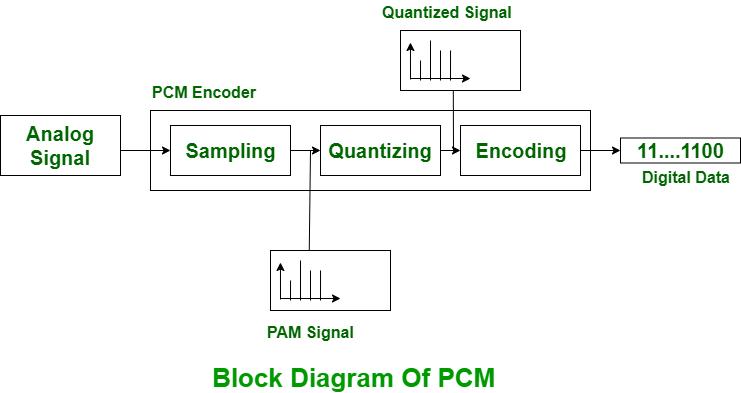
\includegraphics[width=0.9\textwidth]{pcm_diagram.png}
    \caption{Графики}
\end{figure}

\vspace{0.5em}

\textbf{MP3 (MPEG-1 Audio Layer III)} — это формат сжатия аудио с потерями, основанный на психоакустической модели.  
Он удаляет компоненты звука, менее заметные человеческому слуху, и применяет дополнительные методы кодирования, что существенно уменьшает размер файла.  

\vspace{0.5em}

Для конвертации между этими форматами можно использовать библиотеку pydub в Python. А для конвертации MP3 в WAV можно использовать ffmpeg.

\begin{lstlisting}[language=C++, caption=Код на C++ для чтения PCM файла]
int16_t *read_pcm(const char *filename, size_t *sample_count)
{
    FILE *file = fopen(filename, "rb");
    
    fseek(file, 0, SEEK_END);
    long file_size = ftell(file);
    fseek(file, 0, SEEK_SET);
    printf("file_size = %ld\n", file_size);
    
    *sample_count = file_size / sizeof(int16_t);
    int16_t *samples = (int16_t *)malloc(file_size);
    size_t sf = fread(samples, sizeof(int16_t), *sample_count, file);
    
    if (sf == 0){
        printf("file %s empty!", filename);
    }
    
    fclose(file);
    
    return samples;
}
\end{lstlisting}

\section*{Выполнение}

Для начала, я написал код для конвертации mp3 файла в pcm формат с помощью pydub.

\begin{lstlisting}[language=python, caption=Код на python для конвертации mp3 в pcm]
import numpy as np
import librosa
from pydub import AudioSegment

def mp3_to_pcm(src_path, dst_path, sample_rate=44100):
    audio_data, sr = librosa.load(src_path, sr=sample_rate, mono=False)
    if audio_data.ndim > 1:
        audio_data = audio_data.T.flatten()
    pcm_array = np.int16(audio_data * 32767)
    pcm_array.tofile(dst_path)

def pcm_to_mp3(pcm_path, output_path, channels=2, sample_rate=44100, bitrate="160k"):
    raw_audio = np.fromfile(pcm_path, dtype=np.int16)
    sound = AudioSegment(
        data=raw_audio.tobytes(),
        sample_width=2,
        frame_rate=sample_rate,
        channels=channels
    )
    sound.export(output_path, format="mp3", bitrate=bitrate)

print("""PCM->MP3: 0
MP3->PCM: 1""")
ans = int(input("Выберите режим: "))
if ans == 1:
    mp3_to_pcm("../1.mp3", "../1.pcm")
else:
    pcm_to_mp3("../2.pcm", "../2.mp3")
\end{lstlisting}

Он на выбор преобразует mp3 файл в pcm или наоборот. Используем его перед началом экспериментов.
В main.cpp я добавил чтение pcm файла и заполнение буфера прочитанными значениями.

\begin{lstlisting}[language=C++, caption=Заполнения буфера данными из pcm]
size_t iteration_count = 10;
long long last_time = 0;

FILE* file = fopen("../rx.pcm", "wb");
FILE* file1 = fopen("../tx.pcm", "wb");

for (size_t buffers_read = 0; buffers_read < iteration_count; buffers_read++)
    {
        void *rx_buffs[] = {rx_buffer};
        int flags;        // flags set by receive operation
        long long timeNs; //timestamp for receive buffer
        long timeoutUs = 1000000;
        int sr = SoapySDRDevice_readStream(sdr, rxStream, rx_buffs, rx_mtu, &flags, &timeNs, timeoutUs);
        
        printf("Buffer: %lu - Samples: %i, Flags: %i, Time: %lli, TimeDiff: %lli\n", buffers_read, sr, flags, timeNs, timeNs - last_time);
        last_time = timeNs;

        long long tx_time = timeNs + (4 * 1000 * 1000); // на 4 [мс] в будущее

        for(size_t i = 0; i < 8; i++)
        {
            uint8_t tx_time_byte = (tx_time >> (i * 8)) & 0xff;
            tx_buff[2 + i] = tx_time_byte << 4;
        }

        void *tx_buffs[] = {tx_buff};
        if( (buffers_read==2) ){
            flags = SOAPY_SDR_HAS_TIME;
            int st = SoapySDRDevice_writeStream(sdr, txStream, (const void * const*)tx_buffs, tx_mtu, &flags, tx_time, timeoutUs);
            if ((size_t)st != tx_mtu)
            {
                printf("TX Failed: %i\n", st);
            }
        }
        
        fwrite(rx_buffer, 2 * rx_mtu * sizeof(int16_t), 1, file);
        fwrite(tx_buffs, 2 * rx_mtu * sizeof(int16_t), 1, file1);
    }

fclose(file);
\end{lstlisting}

Не забываем закрыть файл через fclose, и получается, что мы записали и отправили наш pcm файл через Pluto SDR, rx\_buffer в file(rx.pcm) и
tx\_buffer в file1(tx.pcm). С помощью нашего кода на python мы можем конвертировать pcm обратно в mp3, чтобы прослушать, полученные mp3 получились искаженными.
Если скрестить две Pluto SDR, одновременно начать отправку сэплов, то получится эффект наложения сигналов. У нас с одногруппником получилось так, что
одновременно были слышны 2 песни.

\section*{Вывод}
Я научился переводить файлы из mp3 в pcm и обратно, записывать их в буфер Pluto SDR, отправлять их и получать, полученные файлы быле конвертированы обратно
в mp3 для того чтобы прослушать, что получилось передать.

\end{document}